%%%%%%%%%%%%%%%%%%%%%%%%%%%%%%%%%%%%%%%%%%%%%%%%%%%%%%%%%%%%%%%%%%%%%
%% This is a (brief) model paper using the achemso class
%% The document class accepts keyval options, which should include
%% the target journal and optionally the manuscript type.
%%%%%%%%%%%%%%%%%%%%%%%%%%%%%%%%%%%%%%%%%%%%%%%%%%%%%%%%%%%%%%%%%%%%%
\documentclass[journal=jpcbfk,manuscript=article]{achemso}

%%%%%%%%%%%%%%%%%%%%%%%%%%%%%%%%%%%%%%%%%%%%%%%%%%%%%%%%%%%%%%%%%%%%%
%% Place any additional packages needed here.  Only include packages
%% which are essential, to avoid problems later. Do NOT use any
%% packages which require e-TeX (for example etoolbox): the e-TeX
%% extensions are not currently available on the ACS conversion
%% servers.
%%%%%%%%%%%%%%%%%%%%%%%%%%%%%%%%%%%%%%%%%%%%%%%%%%%%%%%%%%%%%%%%%%%%%
\usepackage[version=3]{mhchem} % Formula subscripts using \ce{}
%\usepackage[obeyFinal]{easy-todo}
\usepackage{rotating}
\usepackage{epstopdf}
%%%%%%%%%%%%%%%%%%%%%%%%%%%%%%%%%%%%%%%%%%%%%%%%%%%%%%%%%%%%%%%%%%%%%
%% If issues arise when submitting your manuscript, you may want to
%% un-comment the next line.  This provides information on the
%% version of every file you have used.
%%%%%%%%%%%%%%%%%%%%%%%%%%%%%%%%%%%%%%%%%%%%%%%%%%%%%%%%%%%%%%%%%%%%%
%%\listfiles

%%%%%%%%%%%%%%%%%%%%%%%%%%%%%%%%%%%%%%%%%%%%%%%%%%%%%%%%%%%%%%%%%%%%%
%% Place any additional macros here.  Please use \newcommand* where
%% possible, and avoid layout-changing macros (which are not used
%% when typesetting).
%%%%%%%%%%%%%%%%%%%%%%%%%%%%%%%%%%%%%%%%%%%%%%%%%%%%%%%%%%%%%%%%%%%%%
\newcommand*\mycommand[1]{\texttt{\emph{#1}}}

%%%%%%%%%%%%%%%%%%%%%%%%%%%%%%%%%%%%%%%%%%%%%%%%%%%%%%%%%%%%%%%%%%%%%
%% Meta-data block
%% ---------------
%% Each author should be given as a separate \author command.
%%
%% Corresponding authors should have an e-mail given after the author
%% name as an \email command. Phone and fax numbers can be given
%% using \phone and \fax, respectively; this information is optional.
%%
%% The affiliation of authors is given after the authors; each
%% \affiliation command applies to all preceding authors not already
%% assigned an affiliation.
%%
%% The affiliation takes an option argument for the short name.  This
%% will typically be something like "University of Somewhere".
%%
%% The \altaffiliation macro should be used for new address, etc.
%% On the other hand, \alsoaffiliation is used on a per author basis
%% when authors are associated with multiple institutions.
%%%%%%%%%%%%%%%%%%%%%%%%%%%%%%%%%%%%%%%%%%%%%%%%%%%%%%%%%%%%%%%%%%%%%
%\author{Andrew N. Other}
%\altaffiliation{A shared footnote}
%\author{Fred T. Secondauthor}
%\altaffiliation{Current address: Some other place, Othert\"own,
%Germany}
%\author{I. Ken Groupleader}
%\altaffiliation{A shared footnote}
%\email{i.k.groupleader@unknown.uu}
%\phone{+123 (0)123 4445556}
%\fax{+123 (0)123 4445557}
%\affiliation[Unknown University]
%{Department of Chemistry, Unknown University, Unknown Town}
%\alsoaffiliation[Second University]
%{Department of Chemistry, Second University, Nearby Town}
%\author{Susanne K. Laborator}
%\email{s.k.laborator@bigpharma.co}
%\affiliation[BigPharma]
%{Lead Discovery, BigPharma, Big Town, USA}
%\author{Kay T. Finally}
%\affiliation[Unknown University]
%{Department of Chemistry, Unknown University, Unknown Town}
%\alsoaffiliation[Second University]
%{Department of Chemistry, Second University, Nearby Town}

\author{Alexandru Botan}
%\affiliation{The authors are listed in alphaphetical order.}
%\affiliation{The author list is not completed.}
\affiliation[Lyon CNRS]{Institut Lumi\`ere Mati\`ere, UMR5306 Universit\'e Lyon 1-CNRS, Universit\'e de Lyon 69622 Villeurbanne, France}
%
%\author{Andrea Catte}
%\affiliation{University of East Anglia, Norwich, United Kingdom}
\author{Fernando Favela-Rosales}
\affiliation[Mexico]{Departamento de F\'isica, Centro de Investigaci\'on y de Estudios Avanzados del IPN, Apartado Postal 14-740, 07000 M\'exico D.F., M\'exico}
\author{Patrick F. J. Fuchs}
\affiliation[CNRS Paris]{Institut Jacques Monod, CNRS, Universit\'e Paris Diderot, Sorbonne Paris Cit\'e, Paris, France}
%\alsoaffiliation[Diderot University]
%{Institut Jacques Monod, CNRS UMR 7592, Universit{\'e} Paris Diderot, Sorbonne Paris Cit{\'e}, Paris, France}
\author{Matti Javanainen}
\affiliation[Tampere University of Technology]
{Department of Physics, Tampere University of Technology, Tampere, Finland}
\author{Matej Kandu\v{c}}
\affiliation[Freie Universit\"{a}t Berlin] 
{Fachbereich Physik, Freie Universitat Berlin, Berlin, Germany}
\author{Waldemar Kulig}
\affiliation[Tampere University of Technology]
{Department of Physics, Tampere University of Technology, Tampere, Finland}
\author{Antti Lamberg}
\affiliation[Kyoto University]
{Department of Chemical Engineering, Kyoto University, Kyoto, Japan}
\author{Claire Loison}
\affiliation[Lyon CNRS]{Institut Lumi\`ere Mati\`ere, UMR5306 Universit\'e Lyon 1-CNRS, Universit\'e de Lyon 69622 Villeurbanne, France}
\author{Alexander Lyubartsev}
\affiliation[Stockholm University]
{Division of Physical Chemistry, Department of Materials and Environmental Chemistry, Stockholm University, S-106 91 Stockholm, SWEDEN}
\author{Markus S. Miettinen}
\affiliation[Freie Universit\"{a}t Berlin] 
{Fachbereich Physik, Freie Universit\"at Berlin, Berlin, Germany}
\author{Luca Monticelli}
\affiliation[IBCP] 
{Institut de Biologie et Chimie des Prot\'eines (IBCP), CNRS UMR 5086, Lyon, France}
\author{Jukka M{\"a}{\"a}tt{\"a}}
\affiliation[Aalto University]
{Aalto University, Espoo, Finland}
\author{O. H. Samuli Ollila} 
\email{samuli.ollila@aalto.fi.}
\affiliation[Aalto University]
{Aalto University, Espoo, Finland}
\author{Marius Retegan}
\affiliation[Max Planck]
{Max Planck Institute for Chemical Energy Conversion, Mulheim an der Ruhr, Germany}
\author{Tomasz Rog}
\affiliation[Tampere University of Technology]
{Department of Physics, Tampere University of Technology, Tampere, Finland}
\author{Hubert Santuz}
\affiliation[INSERM]
{INSERM, UMR\_S 1134, DSIMB, Paris, France}
\alsoaffiliation[Diderot]
{Universit\'e Paris Diderot, Sorbonne Paris Cit\'e, UMR\_S 1134, Paris, France}
\alsoaffiliation[INTS]
{Institut National de la Transfusion Sanguine (INTS), Paris, France}
\alsoaffiliation[Labex]
{Laboratoire d'Excellence GR-Ex, Paris, France}
\author{Joona Tynkkynen}
\affiliation[Tampere University of Technology]
{Department of Physics, Tampere University of Technology, Tampere, Finland}



%%%%%%%%%%%%%%%%%%%%%%%%%%%%%%%%%%%%%%%%%%%%%%%%%%%%%%%%%%%%%%%%%%%%%
%% The document title should be given as usual. Some journals require
%% a running title from the author: this should be supplied as an
%% optional argument to \title.
%%%%%%%%%%%%%%%%%%%%%%%%%%%%%%%%%%%%%%%%%%%%%%%%%%%%%%%%%%%%%%%%%%%%%
\title[An \textsf{achemso} demo]
  {Towards atomistic resolution structure of phosphatidylcholine headgroup and glycerol backbone at different ambient conditions\footnote{Publication about results presented in the NMRlipids project}}

%%%%%%%%%%%%%%%%%%%%%%%%%%%%%%%%%%%%%%%%%%%%%%%%%%%%%%%%%%%%%%%%%%%%%
%% Some journals require a list of abbreviations or keywords to be
%% supplied. These should be set up here, and will be printed after
%% the title and author information, if needed.
%%%%%%%%%%%%%%%%%%%%%%%%%%%%%%%%%%%%%%%%%%%%%%%%%%%%%%%%%%%%%%%%%%%%%
\abbreviations{IR,NMR,UV}
\keywords{American Chemical Society, \LaTeX}

%%%%%%%%%%%%%%%%%%%%%%%%%%%%%%%%%%%%%%%%%%%%%%%%%%%%%%%%%%%%%%%%%%%%%
%% The manuscript does not need to include \maketitle, which is
%% executed automatically.
%%%%%%%%%%%%%%%%%%%%%%%%%%%%%%%%%%%%%%%%%%%%%%%%%%%%%%%%%%%%%%%%%%%%%
\begin{document}

%%%%%%%%%%%%%%%%%%%%%%%%%%%%%%%%%%%%%%%%%%%%%%%%%%%%%%%%%%%%%%%%%%%%%
%% The "tocentry" environment can be used to create an entry for the
%% graphical table of contents. It is given here as some journals
%% require that it is printed as part of the abstract page. It will
%% be automatically moved as appropriate.
%%%%%%%%%%%%%%%%%%%%%%%%%%%%%%%%%%%%%%%%%%%%%%%%%%%%%%%%%%%%%%%%%%%%%
\begin{tocentry}

%\begin{figure}[]
%  \centering
  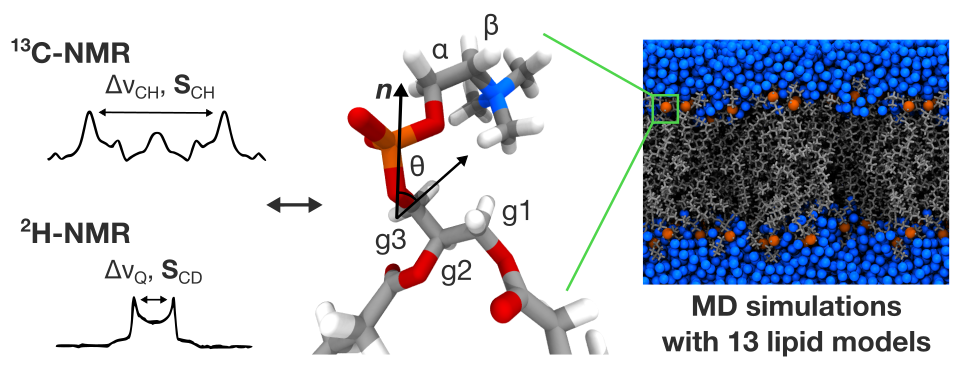
\includegraphics[width=9cm]{../Fig/TOCfinal.png}

%  \caption{\label{POPCstructure}
%    Chemical structure of  1-palmitoyl-2-oleoylphosphatidylcholine (POPC).}
  
%\end{figure}
%Some journals require a graphical entry for the Table of Contents.
%This should be laid out ``print ready'' so that the sizing of the
%text is correct.

%Inside the \texttt{tocentry} environment, the font used is Helvetica
%8\,pt, as required by \emph{Journal of the American Chemical
%Society}.

%The surrounding frame is 9\,cm by 3.5\,cm, which is the maximum
%permitted for  \emph{Journal of the American Chemical Society}
%graphical table of content entries. The box will not resize if the
%content is too big: instead it will overflow the edge of the box.

%This box and the associated title will always be printed on a
%separate page at the end of the document.

\end{tocentry}

%%%%%%%%%%%%%%%%%%%%%%%%%%%%%%%%%%%%%%%%%%%%%%%%%%%%%%%%%%%%%%%%%%%%%
%% The abstract environment will automatically gobble the contents
%% if an abstract is not used by the target journal.
%%%%%%%%%%%%%%%%%%%%%%%%%%%%%%%%%%%%%%%%%%%%%%%%%%%%%%%%%%%%%%%%%%%%%
\begin{abstract}
Phospholipids are essential building blocks of biological membranes.
Despite of vast amount of very accurate experimental data, the atomistic resolution structures sampled by the glycerol backbone and choline headgroup
in phoshatidylcholine bilayers are not known. Atomistic resolution molecular dynamics simulations 
have the potential to resolve the structures, and to give an arrestingly intuitive interpretation of the experimental data---but only if the simulations
reproduce the data within experimental accuracy.
In the present work, we simulated phosphatidylcholine (PC) lipid bilayers with 13 different
atomistic models, and compared simulations with NMR experiments in terms of the highly structurally sensitive C--H bond vector order
parameters. Focusing on the glycerol backbone and choline headgroups, 
we showed that the order parameter comparison can be used to judge the atomistic resolution structural accuracy of the models.
Accurate models, in turn, allow molecular dynamics simulations to be used as an interpretation tool that translates these NMR data
into a dynamic three dimensional representation of biomolecules in biologically relevant conditions.
In addition to lipid bilayers in fully hydrated conditions, we reviewed previous experimental
data for dehydrated bilayers and cholesterol-containing bilayers, and interpreted them with simulations.
Although none of the existing models reached experimental accuracy, by critically comparing them we were able to distill relevant chemical information:
(1) increase of choline order parameters indicates the P--N vector tilting more parallel to the membrane,
and (2) cholesterol induces only minor changes to the PC (glycerol backbone) structure.
This work has been done as a fully open collaboration, using \url{nmrlipids.blogspot.fi} as a
communication platform; all the scientific contributions were made publicly on this blog.
During the open research process, the repository holding our simulation trajectories and files
(\url{https://zenodo.org/collection/user-nmrlipids}) has become the most extensive
publicly available collection of molecular dynamics simulation trajectories of lipid bilayers.
\end{abstract}

%%%%%%%%%%%%%%%%%%%%%%%%%%%%%%%%%%%%%%%%%%%%%%%%%%%%%%%%%%%%%%%%%%%%%
%% Start the main part of the manuscript here.
%%%%%%%%%%%%%%%%%%%%%%%%%%%%%%%%%%%%%%%%%%%%%%%%%%%%%%%%%%%%%%%%%%%%%


\section{Introduction}

Phospholipids containing various polar headgroups and acyl chains are essential building blocks of 
biological membranes. Lamellar phospholipid bilayer structures have been widely studied with various experimental 
and theoretical techniques as a simple model for cellular membranes~\cite{lipowsky95,tieleman97,klauda08,edholm08,tieleman10,piggot12,rabinovich13,marsh13}. 
Phospholipid molecules are composed of hydrophobic acyl chains connected by a glycerol backbone to a hydrophilic headgroup;
see Fig.~\ref{POPCstructure} for the structure of 1-palmitoyl-2-oleoyl\-phosphatidyl\-choline (POPC).
The behaviour of the acyl chains in a lipid bilayer is relatively well understood~\cite{Israelachvili80,lipowsky95,tieleman97,klauda08,edholm08,tieleman10,marsh13}. 
The conformations sampled by the glycerol backbone and choline in a fluid bilayer are, however, not fully 
resolved as even the most accurate scattering and Nuclear Magnetic Resonance (NMR)
techniques give only a set of values that the structure has to fulfill, but
there is no unique way to derive the actual structure from them~\cite{seelig77b,skarjune79,Israelachvili80,jacobs80,davis83,strenk85,akutsu91,hong95b,hong96,semchyschyn04}.
Some structural details have been extracted from crystal structures, $^1$H NMR studies, and Raman spectroscopy~\cite{hauser80,hauser81,hauser81b,akutsu81b,pascher92,hauser88,marsh06},
but general consensus concerning the structures sampled in the fluid state has not been reached~\cite{seelig77b,skarjune79,Israelachvili80,jacobs80,davis83,strenk85,hauser88,akutsu91,hong95b,hong96,semchyschyn04,marsh06}. 
Importantly, the structural parameters for the glycerol backbone are similar for various biologically
relevant lipid species (phosphatidylcholine (PC), phosphatidylethanolamine (PE) and phosphatidylglycerol (PG)) 
in various environments~\cite{gally81}, and the structural parameters for the choline headgroup are similar in model membranes and
real cells (mouse fibroblast L-M cell)~\cite{scherer87}.
Thus, resolving the PC-lipid glycerol and choline structures would be 
useful for understanding a wide range of different biological membranes.

Classical atomistic molecular dynamics simulations have been widely used to study  
lipid bilayers~\cite{tieleman97,klauda08,edholm08,tieleman10,piggot12,rabinovich13}. As these models provide an atomistic
resolution description of the whole lipid molecule, they have the potential to solve the glycerol backbone and 
headgroup structures. The experimental C--H bond order parameters
(routinely compared between experiments and simulations for the acyl chains~\cite{tieleman97,klauda08,edholm08,tieleman10,piggot12})
are also known for the glycerol backbone 
(g$_1$, g$_2$, and g$_3$) and choline ($\alpha$ and $\beta$) segments (see Fig.~\ref{POPCstructure} for definitions) and are among the main parameters used in
attempts to derive lipid structures from experimental data~\cite{seelig77b,skarjune79,jacobs80,davis83,akutsu91,hong95b,semchyschyn04}.
Notably, the structures sampled in a simulation that reproduces these 
parameters will automatically comprise an interpretation of the experiments. In other words, such simulations can be considered as an accurate atomistic resolution description of
the behavior of lipid molecules in a bilayer.

Only a few studies~\cite{shinoda97,hogberg08,castro08,klauda10,kapla12,dickson12,poger12,ferreira13,chowdhary13,maciejewski14}
have compared
the glycerol backbone and choline headgroup order parameters between simulations and experiments. 
The main reason probably is that the existing experimental data for the glycerol backbone
and choline headgroups are scattered over many publications and published in a format that is difficult to understand without some NMR expertise. 
In addition to the order parameters, dihedral angles for the glycerol backbone and headgroup estimated 
from experiments~\cite{robinson94,essex94,kothekar96,hyvonen97,shinoda97,duong99}, 
$^{31}$P chemical shift anisotropy~\cite{chowdhary13} and $^{31}$P-$^{13}$C dipolar couplings~\cite{prakash10}
have been used to assess the quality of a simulation model.

In this work, we first review the most relevant experimental data for the glycerol backbone and choline headgroup order parameters
in a phosphatidylcholine lipid bilayer. Then the available atomistic resolution lipid models are carefully compared to the 
experimental data. The comparison reveals that the CHARMM36~\cite{klauda10}, GAFFlipid~\cite{dickson12}, and MacRog~\cite{maciejewski14} models
have the most realistic glycerol backbone and choline structures. We also compare the glycerol backbone and choline 
structures between the most often used (Berger-based) lipid model~\cite{berger97} 
and the best performing models, to demonstrate that by using the 
order parameters we can distinguish the more reasonable structures from the less reasonable ones. However, none of the current models 
is accurate enough to properly resolve the atomistic resolution structures.

In addition to fully hydrated single component lipid bilayers, the glycerol backbone and choline order parameters
have been measured under a large number of changing conditions: hydration level~\cite{bechinger91,ulrich94,dvinskikh05b}, cholesterol content~\cite{brown78,ferreira13},
ion concentration~\cite{brown77,akutsu81,altenbach84,roux90,roux91}, temperature~\cite{gally75}, charged lipid content~\cite{roux90,roux91}, charged surfactant content~\cite{scherer89}, 
drug molecule concentration~\cite{browning82,kelusky84,castro08}, and protein content~\cite{roux89,kuchinka89} (listing only the publications most relevant for this work and the pioneering studies).
Existence of these data allows the comparison of structural responses to varying conditions between simulations and experiments,
in other words, validation of the simulation models and interpretation of the original experiments. 
Here we demonstrate the power of this approach in understanding the behaviour of a bilayer as a function of hydration level and cholesterol content.
Choline headgroup order parameters as function of ion concentration, and their relation to the ion binding affinity, are discussed elsewhere~\cite{ionpaper}.

  \begin{figure}[]
  \centering
  \includegraphics[width=8.6cm]{../Fig/POPCstructure.pdf}

  \caption{\label{POPCstructure}
    Chemical structure of  1-palmitoyl-2-oleoylphosphatidylcholine (POPC).}
  
\end{figure}

\section{Methods}

\subsection{Open collaboration}

This work has been done as a fully open collaboration, using the \url{nmrlipids.blogspot.fi} blog~\cite{nmrlipids}
as a communication platform.
Our approach is inspired by the Polymath project~\cite{gowers09}, however there are some essential differences. 
We started by publishing a manuscript~\cite{ollila13} discussing the glycerol backbone and choline structures 
in a Berger-based model (the most used molecular dynamics simulation model for lipid bilayers).
Simultaneously,  we presented an open invitation for further contributions and discussion on the blog.
All the scientific contributions were made publicly through the blog. Every contributor was offered coauthorship
according to the guidelines defined in the beginning of the project~\cite{creditsPOST};
the acceptance of the offer was based on authors' self-assesment of their scientific contribution.
These contributions are summarized in the Supporting Information. 

Almost all simulation data, including input files for reproduction and trajectories for further analysis, are collected
on our CERN-hosted Zenodo file repository (\url{https://zenodo.org/collection/user-nmrlipids}).
Thus, in addition to the main topic of this manuscript, we present the most extensive publicly available collection of simulation trajectories
for lipid bilayers, opening up numerous possiblities for different analyses with much less effort than previously required.
Further information, such as scripts, figures, and manuscript text files, are available through our GitHub 
repository~\cite{NMRLipidsGit}.% (\url{https://github.com/NMRlipids}). 


\subsection{Order parameters from experiments}\label{expORDp}
The order parameter of a hydrocarbon C--H vector is defined as 
\begin{equation}\label{orderP}
S_{{\rm CH}}=\frac{1}{2}\langle 3 \cos^2 \theta-1 \rangle,
\end{equation} 
where the angle brackets denote an ensemble average over the sampled conformations, and $\theta$ is the angle between the C--H bond and the membrane normal.
The absolute values of order parameters can be measured by detecting quadrupolar splitting with $^2$H NMR~\cite{seelig77c} or by detecting dipolar 
splitting with $^1$H-$^{13}$C NMR~\cite{hong95a,gross97,dvinskikh05a,ferreira13}. The measurements are based on
different physical interactions, and also the connections between order parameter and quadrupolar or dipolar splitting
are different. The absolute values of order parameters from the measured quadrupolar splitting $\Delta \nu_Q$ ($^2$H NMR) are calculated using 
the equation $|S_{{\rm CD}}|=\frac{4}{3} \frac{h}{e^2qQ} \Delta \nu_Q$, where the value for the static quadrupole
splitting constant is estimated from various experiments to be 170~kHz leading to a numerical relation 
$|S_{{\rm CD}}|=0.00784 \times \Delta \nu_Q$~\cite{seelig77c}. 
The absolute values of order parameters from the effective dipolar coupling $d_\mathrm{CH}$ ($^1$H-$^{13}$C NMR) are calculated using the equation
$|S_{{\rm CH}}|=\frac{4\pi\langle r_\mathrm{CH}^3 \rangle}{\hbar \mu_0 \gamma_h \gamma_c} d_\mathrm{CH}$, where
values between 20.2--22.7~kHz are used for $\frac{4\pi\langle r_\mathrm{CH}^3 \rangle}{\hbar \mu_0 \gamma_h \gamma_c}$,
depending on the original authors~\cite{hong95a,gross97,dvinskikh05a,ferreira13}.
The effective dipolar coupling $d_\mathrm{CH}$ is related to the measured dipolar splitting $\Delta \nu_\mathrm{CH}$ 
through a scaling factor that depends on the pulse sequence used in the $^1$H-$^{13}$C NMR experiment~\cite{hong95a,gross97,dvinskikh05a,ferreira13}.
It is important to note that the order parameters measured with different techniques based on different physical interactions are in good agreement
with each other (see Results and Discussion), indicating very high quantitative accuracy of the measurements.
For a more detailed discussion, see Ref.~\citenum{accuracyPOST}. 

The absolute values of order parameters are accessible with both $^2$H NMR and $^1$H-$^{13}$C NMR techniques. 
However, only $^1$H-$^{13}$C NMR techniques allow also the measurement of the sign of the order parameter~\cite{hong95a,hong95b,gross97}. 
The measured sign is negative for almost all the carbons discussed in this work, except for $\alpha$ which is positive~\cite{hong95a,hong95b,gross97}. 
For more detailed discussion about the determination of the sign of the order parameters, see Ref.~\citenum{signpost}. 

For most CH$_2$ segments in a fluid phospholipid bilayer, the order parameters of both hydrogens are equal.
However, in some cases (e.g., g$_1$, g$_3$, and  C$_2$ carbon in the \textit{sn}-2 chain) the two order parameters are not equal;
this  can be observed with both $^2$H NMR and $^1$H-$^{13}$C NMR techniques. In the present work,
to avoid confusion with the dipolar and quadrupolar splittings in NMR terminology,
we call the phenomenon of unequal order parameters for hydrogens attached to the same carbon {\it forking}. 
Forking has been studied in detail with $^2$H NMR techniques by deuterating the R or S position in CH$_2$ segment, and
the studies show that it arises from differently sampled orientations of the two C--H bonds, not from two 
separate populations of lipid conformations~\cite{engel81,gally81}.


\subsection{Order parameters from simulations}
The order parameters from simulations were calculated directly using the definition of Eq.~\ref{orderP}.
For the united atom models, the hydrogen positions were generated 
post-simulationally from the positions of the heavy atoms and the known hydrocarbon geometries.
The statistical error was estimated based on the assumption that different lipids are statistically independent 
entities (which should be the case in fluid phase):
The time average of a given order parameter was first calculated separately for each lipid,
and the standard error of the mean over these time averages then taken as the error bar for this order parameter.

It has been pointed out that the sampling of individual dihedral angles might be very
slow compared to the typical (100~ns) simulation timescales~\cite{vogel12}.
After 200~ns, however, even the slowest rotational correlation function of a C--H bond  (g$_1$) reaches
a plateau ($S_\mathrm{CH}^2$) in the Berger-POPC-07 model~\cite{ollila07a}---and, notably,
the dynamics of this segment have been shown to be significantly slower in simulations
than in experiments~\cite{ferreira15}.
In practise,
due to averaging over different lipid molecules,
less than 200~ns of simulation data should be enough for the order parameter calculation;
if the sampling within typical simulation times
is not enough for the convergence of the order parameters,
then the simulation model in question has unphysically slow dynamics.





\subsection{Simulated systems}
All simulations are ran with a standard setup for a planar lipid bilayer in zero tension and constant temperature
with periodic boundary conditions in all directions by using the GROMACS software package~\cite{hess08} 
(version numbers 4.5.X--4.6.X), LAMMPS~\cite{plimpton95}, MDynaMix~\cite{Lyubartsev00} or NAMD~\cite{phillips05}.
The number of molecules, simulation temperatures and the length of simulations of all the simulated systems 
are listed in Tables~\ref{systems},~\ref{systemsDEHYD} and~\ref{systemsCHOL}. Full simulation
details are given in the Supporting Information (SI) or in the original publications in case the
data is used previously therein. All simulation parameters were set as close to the original 
parametrization works as possible.
Additionally, the files related to the simulations and the resulting trajectories are publicly
available for almost all systems in the Zenodo collection \url{https://zenodo.org/collection/user-nmrlipids}. 
The references pointing to simulation details and files are also listed in Tables~\ref{systems},~\ref{systemsDEHYD} and~\ref{systemsCHOL}.

\begin{sidewaystable}[]
\centering
\caption{Fully hydrated single component lipid bilayer systems simulated for Fig.~\ref{HGorderparameters}:
  1,2-dimyristoyl-sn-glycero-3-phosphocholine (DMPC),
  dilauroylphosphatidylcholine (DLPC),
  dipalmitoylphosphatidylcholine (DPPC), and
  1-palmitoyl-2-oleoylphosphatidylcholine (POPC).
The {\bf bolded} systems were used also for Fig.~\ref{HGorderparameters2}.
$^a$ Number of lipid molecules.
$^b$ Number of water molecules.
$^c$ Temperature.
$^d$ Total simulation time.
$^e$ Time used for analysis.
$^f$ Reference link for the downloadable simulation files;
     the data sets marked with $^*$ also include a part of the trajectory.
$^g$ Reference for the full simulation details;
     the original publication is cited if simulation data from previously published work has been directly used,
     for other systems the simulation details are given in the Supporting Information.
$^h$ Magnitudes from Fig.~S4 of Klauda et al.~\cite{klauda10}, signs matched to our simulations.
$^i$ Magnitudes from Fig.~9 of Dickson et al.~\cite{dickson12}, signs matched to our simulations.
}\label{systems}
\begin{tabular}{l l r r r r r c c}
%\hline
Force field & lipid & $^a$N$_{\rm l}$   &  $^b$N$_{\rm w}$ &  $^c$T (K)  &  $^d$t$_{{\rm sim}}$(ns) &  $^e$t$_{{\rm anal}}$ (ns) &  $^f$Files  &  $^g$Details\\
\hline
Berger-DMPC-04~\cite{gurtovenko04} & DMPC & 128 & 5097 & 323 & 130 & 100 & [\citenum{dmpcFILES}]$^*$       & [\citenum{miettinen09}] \\
Berger-DPPC-98~\cite{marrink98}    & DPPC &  72 & 2864 & 323 & 60 & 30 & [\citenum{bergerDPPCfiles}]$^*$ & SI \\
{\bf
Berger-POPC-07}~\cite{ollila07a}   & POPC & 128 & 7290 & 298 & 270 & 240 & [\citenum{bergerFILESpopc}]$^*$ & [\citenum{ferreira15}] \\
CHARMM36~\cite{klauda10}  & DPPC &  72 & 2189 & 323 &  30 &  25 & [\citenum{charmmFILESdppc}]$^*$    & SI \\
CHARMM36~\cite{klauda10}  & DPPC &  72 & 2189 & 323 &  130  & - & -   & [\citenum{klauda10}]$^h$  \\
CHARMM36~\cite{klauda10}  & POPC &  72 & 2242 & 303 &  30 &  20 & [\citenum{charmm36filesSHORT}]$^*$ & SI \\
{\bf
CHARMM36}~\cite{klauda10} & POPC & 128 & 5120 & 303 & 200 & 100 & [\citenum{charmm36files}]$^*$      & SI \\
MacRog~\cite{kulig15b}  & POPC & 288 & 12600 & 310 & 100 &  80 & [\citenum{macrogFILES}]$^*$      & SI  \\
{\bf
MacRog}~\cite{kulig15b} & POPC & 128 &  6400 & 310 & 400 & 200 & [\citenum{macrogCHOLfiles}]$^*$  & SI  \\
MacRog~\cite{kulig15b}  & POPC & 288 & 14400 & 310 &  90 &  40 & [\citenum{macrogdehydFILES}]$^*$ & SI  \\
GAFFlipid~\cite{dickson12}   & DPPC &  72 & 2197 & 323 &  90 & 50 & [\citenum{GAFFlipidFILESdppc}]$^*$ & SI \\
GAFFlipid~\cite{dickson12}   & DPPC &  72 & 2167 & 323 & 250 &  250 & -   &  [\citenum{dickson12}]$^i$   \\
{\bf
GAFFlipid}~\cite{dickson12}  & POPC & 126 & 3948 & 303 & 137 & 32 & [\citenum{GAFFlipidFILES}]$^*$ & SI \\
Lipid14 \cite{dickson14}         & POPC  & 72 & 2234 & 303 & 100 & 50  & [\citenum{lipid14files}]$^*$ & SI \\
Poger \cite{poger10}             & DPPC  & 128 & 5841 & 323 & 2$\times$100 & 2$\times$50 & [\citenum{pogerFILESpme1,pogerFILESpme2}]$^*$ & SI \\
Slipids \cite{jambeck12}          & DPPC & 128 & 3840 & 323 & 150 & 100 & [\citenum{slipidsFILES}]$^*$ & SI \\
Slipids \cite{jambeck12b}          & POPC & 128 & 5120 & 303 & 200 & 150 & [\citenum{slipidsFILESpopc}]$^*$ & SI \\
Kukol \cite{kukol09}          & POPC   & 512 & 20564 & 298 & 50 & 30  & [\citenum{kukolFILES}]$^*$ & SI \\
Chiu \cite{chiu09}      & POPC  & 128 & 3552  & 298 & 56 & 50  & [\citenum{chiuFILES}]$^*$ & SI \\
H\"ogberg08 \cite{hogberg08}    & DMPC &  98 & 3840 & 303 &  75 & 50 &  [\citenum{hogbergDMPCfiles}]$^*$ & [\citenum{hogberg08}] \\
H\"ogberg08 \cite{rabinovich14} & POPC & 128 & 3840 & 303 & 100 & 80 &  [\citenum{hogbergPOPCfiles}]$^*$ & [\citenum{rabinovich14}]  \\
Ulmschneiders \cite{Ulmschneider09}    & POPC  & 128 & 3328 & 310 & 100 & 50 & [\citenum{ulmschneiderFILES}]$^*$ & SI \\
Tj\"ornhammar14 \cite{tjornhammar14}   & DPPC  & 144 & 7056 & 323 & 200 & 100 & [\citenum{tjornhammarfiles}]$^*$ & [\citenum{tjornhammar14}] \\
Botan-CHARMM36-UA~\cite{henin08} & DLPC & 128 & 3840 & 323 & 30 & 20 & [\citenum{charmmUAfiles}]        & SI \\
Lee-CHARMM36-UA~\cite{lee14}     & DPPC &  72 & 2189 & 323 & 70 & 50 & [\citenum{charmmUAfilesLEE}]$^*$ & SI \\
\end{tabular}
\end{sidewaystable} 

\begin{table}[htb]
\centering
\caption{Simulated single component lipid bilayers with varying hydration levels. The simulation file data sets marked with $^*$ include also part of the trajectory.
$^a$ Water/lipid molar ratio
$^b$ The number of lipid molecules
$^c$ The number of water molecules
$^d$ Simulation temperature
$^e$ The total simulation time
$^f$ Time frames used in the analysis
$^g$ Reference link for the downloadable simulation files
$^h$ Reference for the full simulation details
}\label{systemsDEHYD}
\begin{tabular}{c c c c c c c c c c}
%\hline
Force field & lipid & $^a$n (w/l)   & $^b$N$_{\rm l}$   &  $^c$N$_{\rm w}$ & $^d$T (K)  & $^e$t$_{{\rm sim}}$(ns)  & $^f$t$_{{\rm anal}}$ (ns)& $^g$Files  &  $^h$Details\\
\hline
Berger-POPC-07~\cite{ollila07a}          &   POPC & 57  &128 & 7290  & 298  & 270 & 240 & [\citenum{bergerFILESpopc}]$^*$ & SI \\
                                        &   POPC & 7  &128 & 896   & 298  & 60 & 50 & [\citenum{bergerDEHYDfiles}]$^*$ & SI \\
Berger-DLPC-13~\cite{kanduc13}          &   DLPC & 28  &72 & 2016  & 300  & 80 & 60 & [\citenum{bergerFILESdlpc28}]$^*$ & [\citenum{kanduc13}] \\
                                 &   DLPC & 24  &72 & 1728  & 300  & 80 & 60 & [\citenum{bergerFILESdlpc24}]$^*$ & [\citenum{kanduc13}] \\
                                 &   DLPC & 20  &72 & 1440  & 300  & 80 & 60 & [\citenum{bergerFILESdlpc20}]$^*$ & [\citenum{kanduc13}] \\
                                 &   DLPC & 16  &72 & 1152  & 300  & 80 & 60 & [\citenum{bergerFILESdlpc16}]$^*$ & [\citenum{kanduc13}] \\
                                 &   DLPC & 12  &72 & 864  & 300  & 80 & 60 & [\citenum{bergerFILESdlpc12}]$^*$ & [\citenum{kanduc13}] \\
                                 &   DLPC & 8  &72 & 576  & 300  & 80 & 60 & [\citenum{bergerFILESdlpc8}]$^*$ & [\citenum{kanduc13}] \\
                                 &   DLPC & 4  &72 & 288  & 300  & 80 & 60 & [\citenum{bergerFILESdlpc4}]$^*$ & [\citenum{kanduc13}] \\
CHARMM36\cite{klauda10}          & POPC   & 40 & 128 &  5120   & 303 & 150 & 100  & [\citenum{charmm36files}]$^*$   & SI \\
                                 & POPC   & 31  & 72  &  2242 & 303 & 30 & 20 & [\citenum{charmm36filesSHORT}]$^*$ & SI \\
                               & POPC   & 15 & 72 &  1080  & 303 & 59 & 40 & [\citenum{charmm36files15wPERl}]$^*$ & SI \\
                            & POPC   & 7  & 72  &  504  & 303 & 60 & 20 & [\citenum{charmm36files7wPERl}]$^*$ & SI \\
MacRog\cite{kulig15b}     & POPC   & 50 & 288  & 14400 & 310 & 90 & 40 & [\citenum{macrogdehydFILES}]$^*$ & SI \\
                               & POPC   & 44 & 288  & 12600 & 310 & 100 & 80 & [\citenum{macrogFILES}]$^*$ & SI \\
                               & POPC   & 25 & 288  & 7200 & 310 & 100 & 50 & [\citenum{macrogdehydFILES}]$^*$ & SI \\
                                & POPC   & 20 & 288  & 5760 & 310 & 100 & 50 & [\citenum{macrogdehydFILES}]$^*$ & SI \\
                                & POPC   & 15 & 288  & 4320 & 310 & 100 & 50 & [\citenum{macrogdehydFILES}]$^*$ & SI \\
                                & POPC   & 10 & 288  & 2880 & 310 & 100 & 50 & [\citenum{macrogdehydFILES}]$^*$ & SI \\
                                & POPC   & 5 & 288   & 1440 & 310 & 100 & 50 & [\citenum{macrogdehydFILES}]$^*$ & SI \\
GAFFlipid\cite{dickson12}      & POPC   & 31& 126  & 3948  & 303 & 137 & 32 & [\citenum{GAFFlipidFILES}]$^*$ & SI  \\
                               & POPC   & 7& 126  & 896   & 303 & 130 & 40 & [\citenum{gaffDEHYDfiles}]$^*$ & SI \\
\end{tabular}
\end{table} 

\begin{sidewaystable}[]
\centering
\caption{Simulated lipid bilayers containing cholesterol. The simulation file data sets marked with $^*$ include also part of the trajectory.
$^a$ The number of lipid molecules
$^b$ The number of cholesterol molecules
$^c$ Cholesterol concentration (mol\%)
$^d$ The number of water molecules
$^e$ Simulation temperature
$^f$ The total simulation time
$^g$ Time frames used in the analysis
$^h$ Reference link for the downloadable simulation files
$^i$ Reference for the full simulation details
}\label{systemsCHOL}
\begin{tabular}{c c c c c c c c c c c}
%\hline
Force field & lipid   & $^a$N$_{\rm l}$ & $^b$N$_{\rm chol}$ &$^c$C$_{\rm CHOL}$  &  $^d$N$_{\rm w}$ & $^e$T (K)  & $^f$t$_{{\rm sim}}$(ns)  & $^g$t$_{{\rm anal}}$ (ns)& $^h$Files  &  $^i$Details\\
\hline
Berger-POPC-07~\cite{ollila07a}&   POPC &128 & 0 &0\% & 7290  & 298  & 270 & 240 & [\citenum{bergerFILESpopc}]$^*$ & [\citenum{ferreira15}] \\
/H\"oltje-CHOL-13~\cite{holtje01,ferreira13}   &    & &  &   &   &  &  &  &  \\
                               &   POPC &120 & 8 & 6\% &7290   & 298  & 100 & 80 & [\citenum{bergerFILESpopc7chol}]$^*$ & [\citenum{ferreira13}] \\
                               &   POPC &110 & 18& 14\% & 8481  & 298  & 100 & 80 & [\citenum{bergerFILESpopc15chol}]$^*$ & [\citenum{ferreira13}]  \\
                               &   POPC &84 & 44 & 34\%  & 6794   & 298  & 100 & 80 & [\citenum{bergerFILESpopc34chol}]$^*$ & [\citenum{ferreira13}] \\
                               &   POPC &64 & 64 & 50\% & 10314  & 298  & 100 & 80 & [\citenum{bergerFILESpopc50chol}]$^*$ & [\citenum{ferreira13}] \\
                               &   POPC &50 & 78 & 61\% & 5782   & 298  & 100 & 80 & [\citenum{bergerFILESpopc60chol}]$^*$ & [\citenum{ferreira13}] \\
CHARMM36\cite{klauda10,lim12}   & POPC   & 128& 0& 0\% & 5120  & 303  & 150 & 100 & [\citenum{charmm36files}]$^*$  & SI  \\
                                & POPC   & 512& 0& 0\% & 23943  & 298  & 170 & 100 & [\citenum{charmmPOPC512files}]$^*$  & SI  \\
                                & POPC   & 460& 52& 10\% & 23569  & 298  & 170 & 100 & [\citenum{charmmPOPC512files}]$^*$  & SI  \\
                                & POPC   & 436& 76& 15\% & 23331  & 298  & 170 & 100 & [\citenum{charmmPOPC512files}]$^*$  & SI  \\
                                & POPC   & 100 & 24 & 19\%  &  4960   & 303 & 200 & 100 & [\citenum{charmm36files20perCHOL}]$^*$ & SI \\
                                & POPC   & 410& 102& 20\% & 20972  & 298  & 170 & 100 & [\citenum{charmmPOPC512files}]$^*$  & SI  \\
                                & POPC   & 384& 128& 25\% & 22327  & 298  & 170 & 100 & [\citenum{charmmPOPC512files}]$^*$  & SI  \\
                                & POPC   & 332& 180& 35\% & 21340  & 298  & 170 & 100 & [\citenum{charmmPOPC512files}]$^*$  & SI  \\
                                & POPC   & 256& 256& 50\% & 20334  & 298  & 170 & 100 & [\citenum{charmmPOPC512files}]$^*$  & SI  \\
                               & POPC   & 80 & 80 &50\%  &  4496    & 303 & 200 & 100 & [\citenum{charmm36files50perCHOL}]$^*$ & SI \\
MacRog\cite{kulig15b}     & POPC   & 128 & 0 & 0\% & 6400  & 310 & 400 & 200 & [\citenum{macrogCHOLfiles}]$^*$ & SI \\ 
                          & POPC   & 114  & 14 & 11\% & 6400  & 310  & 400 & 200 & [\citenum{macrogCHOLfiles}]$^*$ & SI    \\
                          & POPC   & 72   & 56 &  44\% & 6400  & 310  & 400 & 200 & [\citenum{macrogCHOLfiles}]$^*$ & SI    \\
                             & POPC   & 64  & 64 & 50\% & 6400  & 310  & 400 & 200 & [\citenum{macrogCHOLfiles}]$^*$ & SI    \\
                             & POPC   & 56   & 72 & 56\% & 6400  & 310  & 400 & 200 & [\citenum{macrogCHOLfiles}]$^*$ & SI    \\
\end{tabular}
\end{sidewaystable} 

\section{Results and Discussion}

\subsection{Full hydration: Experimental order parameters for the glycerol backbone and headgroup}\label{experiments}
The specific deuteration of $\alpha$-, $\beta$- and g$_3$- segments of DPPC has been successful, 
allowing the absolute value order parameter measurements for these segments by $^2$H NMR~\cite{gally75,brown77,brown78,akutsu81}.
In addition, the absolute values of order parameters for all glycerol backbone and choline headgroup segments in egg yolk lecithin~\cite{hong95a},
DMPC~\cite{hong95b,gross97,dvinskikh05a}, DOPC~\cite{warschawski05} and POPC~\cite{warschawski05,ferreira13}
have been measured with several different implementations of $^1$H-$^{13}$C NMR experiments. In addition, the signs of order parameters in some systems
are measured with $^1$H-$^{13}$C NMR techniques~\cite{hong95a,hong95b,gross97}. The experimental values of glycerol backbone 
and choline order parameters from various publications~\cite{gally75,akutsu81,gross97,dvinskikh05a,ferreira13} with the signs measured in~\cite{hong95a,hong95b,gross97} are shown in Fig.~\ref{HGorderparameters}.
\begin{figure}[]
%  \centering
  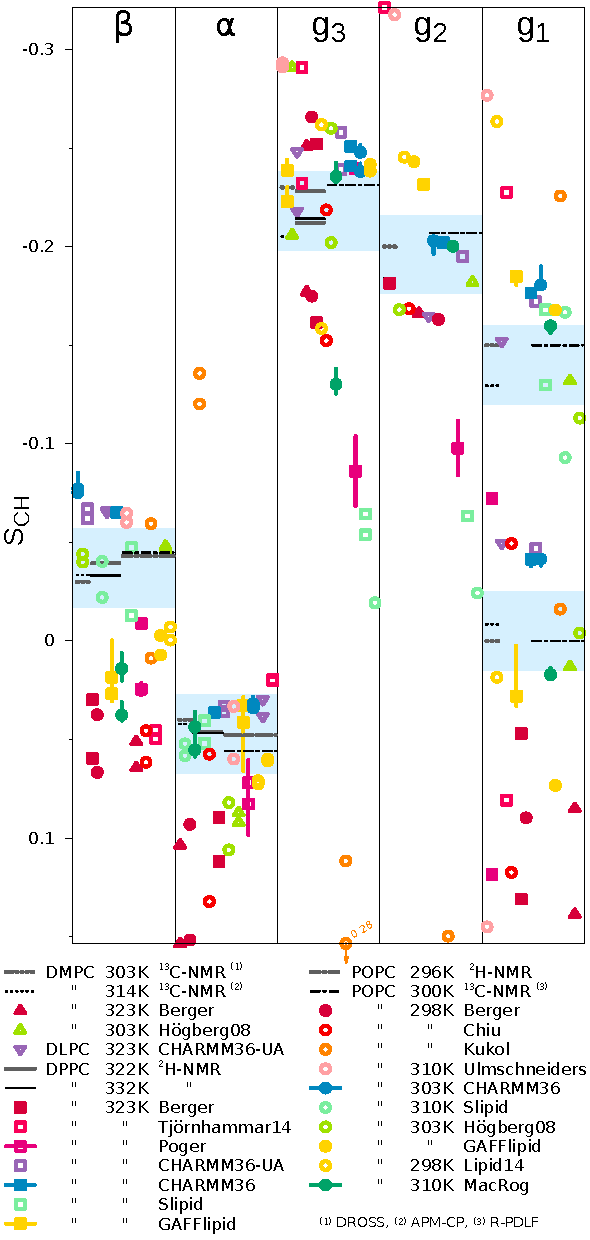
\includegraphics[width=8.6cm]{../DATAreportediINblog/comparisonSorted.pdf}
\newline
  \caption{\label{HGorderparameters}
  Order parameteres from simulations listed in Table~\ref{systems} and experiments for glycerol and choline groups.
The experimental values were taken from the following publications:
 DMPC 303~K from \cite{gross97},
 DMPC 314~K from \cite{dvinskikh05a},
 DPPC 322~K from \cite{gally75},
 DPPC 323~K from \cite{akutsu81},
 POPC 296~K from \cite{bechinger91}, and
 POPC 300~K from \cite{ferreira13}.
  The vertical bars shown for some of the computational values are not error bars, but demonstrate that for 
these systems we had at least two data sets (see Table~\ref{systems});
the ends of the bars mark the extreme values from the sets, and the dot marks their measurement-time-weighted average. 
The interactive version of this figure is available at  https://plot.ly/$\sim$HubertSantuz/72/lipid-force-field-comparison/.
} 
\end{figure}

In general there is a good agreement between the order parameters measured with different experimental NMR techniques: Almost all the 
reported values are within a variation of $\pm$0.02 (which is also the error estimate given by Gross et al.~\cite{gross97}) 
for all fully hydrated PC bilayer, regardless of the variation in their acyl chain composition and temperature.
Exceptions are the somewhat lower order parameters sometimes reported from measurements using $^1$H-$^{13}$C NMR~\cite{hong95a,hong95b,warschawski05}.
These experiments are not shown in Fig.~\ref{HGorderparameters} as the reported error bars are either relatively large~\cite{hong95a,hong95b}, 
or the spectral resolution is quite low and the numerical lineshape simulations have not been used in the analysis~\cite{warschawski05}.
Due to this end, it is highly likely that these reported lower order parameters are due to lower experimental 
accuracy and therefore we exclude them from our discussion. 
For more details, see Ref.~\citenum{accuracyPOST}. 
Motivated by the high experimental reproducibility, we have highlighted in 
Fig.~\ref{HGorderparameters} the subjective sweet spots (light blue areas), within which we expect the calculated absolute 
values of the order parameters of a well-performing force field to fall.

In addition to the numerical values, an important feature of the glycerol backbone is the 
forking (see section~\ref{expORDp}) of the order parameters in g$_1$ and g$_3$ segments, in contrast to the choline segments $\alpha$ and $\beta$. 
The forking in glycerol backbone g$_3$ segment is small ($\approx$ 0.02) 
and some experiments only report the larger value or the average value~\cite{akutsu81,ferreira13}. 
In contrast, forking is significant for the glycerol backbone g$_1$ segment, whose lower order parameter is close to zero and the
larger one has an absolute value of approximately 0.13--0.15. Forking was studied in detail by Gally et al.~\cite{gally81}, who used E. Coli to 
stereospecifically deuterate the different hydrogens attached to the g$_1$ or g$_3$ groups in PE lipids, and measured the order parameters from the lipid 
extract. This experiment gave the lower order parameter when deuterium was in the S position of g$_1$ or R position for g$_3$.
Since the glycerol backbone order parameters are very similar irrespective of the headgroup chemistry (PC,PE and PG) or lipid 
environment~\cite{gally81}, it is reasonable to assume that the stereospecifity measured for the PE lipids
holds also for the PC lipids.

The most detailed experimentally available order parameter information for the glycerol backbone and choline 
segments of POPC bilayer is collected by taking the absolute values from~\cite{ferreira13}, the signs from~\cite{hong95a,hong95b,gross97} 
and the stereospecific labeling from~\cite{gally81}, and shown in Fig.~\ref{HGorderparameters2}.
\begin{figure*}[]
  \centering
  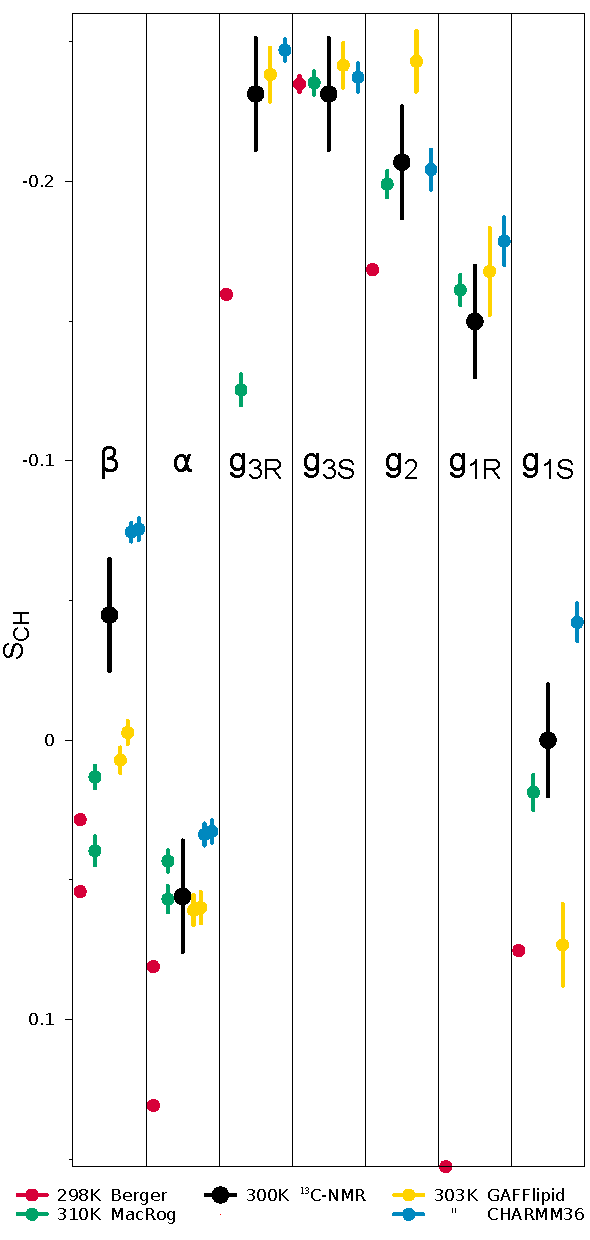
\includegraphics[width=8.6cm]{../Fig/stereospecificOPs.pdf} \\
  \caption{\label{HGorderparameters2}
  Order parameteres for POPC glycerol and choline groups
  from simulations with Berger-POPC-07, MacRog, GAFFlipid, and CHARMM36 force fields
  (the {\bf bolded} systems in Table~\ref{systems})
  together with experimental values.
  The error bars of simulation data are standard errors of mean (see Methods for details).
  The magnitudes for experimental order parameters are taken from Ferreira et al.~\cite{ferreira13},
  the signs are based on the measurements by Hong et al.~\cite{hong95a,hong95b} 
  and Gross et al.~\cite{gross97}, and the R/S labeling is based on the measurements by Gally et al.~\cite{gally81}.
}
\end{figure*}

\subsection{Full hydration: Comparison between simulation models and experiments}

The order parameters of the glycerol backbone and headgroup calculated from different force fields for various lipids have been 
previously compared to experiments~\cite{shinoda97,hogberg08,castro08,klauda10,kapla12,dickson12,poger12,ferreira13,chowdhary13,maciejewski14}. 
The general conclusion from these studies seems to be that the CHARMM based~\cite{hogberg08,klauda10}, GAFFlipid~\cite{dickson12} and
MacRog~\cite{maciejewski14} force fields perform better for the glycerol backbone and headgroup structures than the GROMOS based models~\cite{castro08,kapla12,poger12,ferreira13}.
However, none of the studies exploits the full potential of the available experimental data discussed in previous section, i.e. the quantitative accuracy, known signs and stereospecific labeling of
the experimental order parameters.

To get a general idea of the quality of the glycerol backbone and choline headgroup structures in different models, we calculated 
the order parameters for these parts from thirteen different lipid models (Table~\ref{systems}) and 
plotted the results together with experimental values in Fig.~\ref{HGorderparameters}.
Two criteria were used to judge the quality of the model: there must not be significant  {\bf forking} in the $\alpha$ and $\beta$ carbons,
there must be only moderate forking in the g$_3$ carbon and there must be significant forking in the g$_1$ carbon, the {\bf magnitude}
should be preferably inside to the subjective sweet spots determined from experiments (blue shaded regions in Fig.~\ref{HGorderparameters}).
The results for each force field with respect to the above criteria are summarized in Figure~\ref{FullHydrationComparisonTable}.
\begin{figure}[]
  \centering
  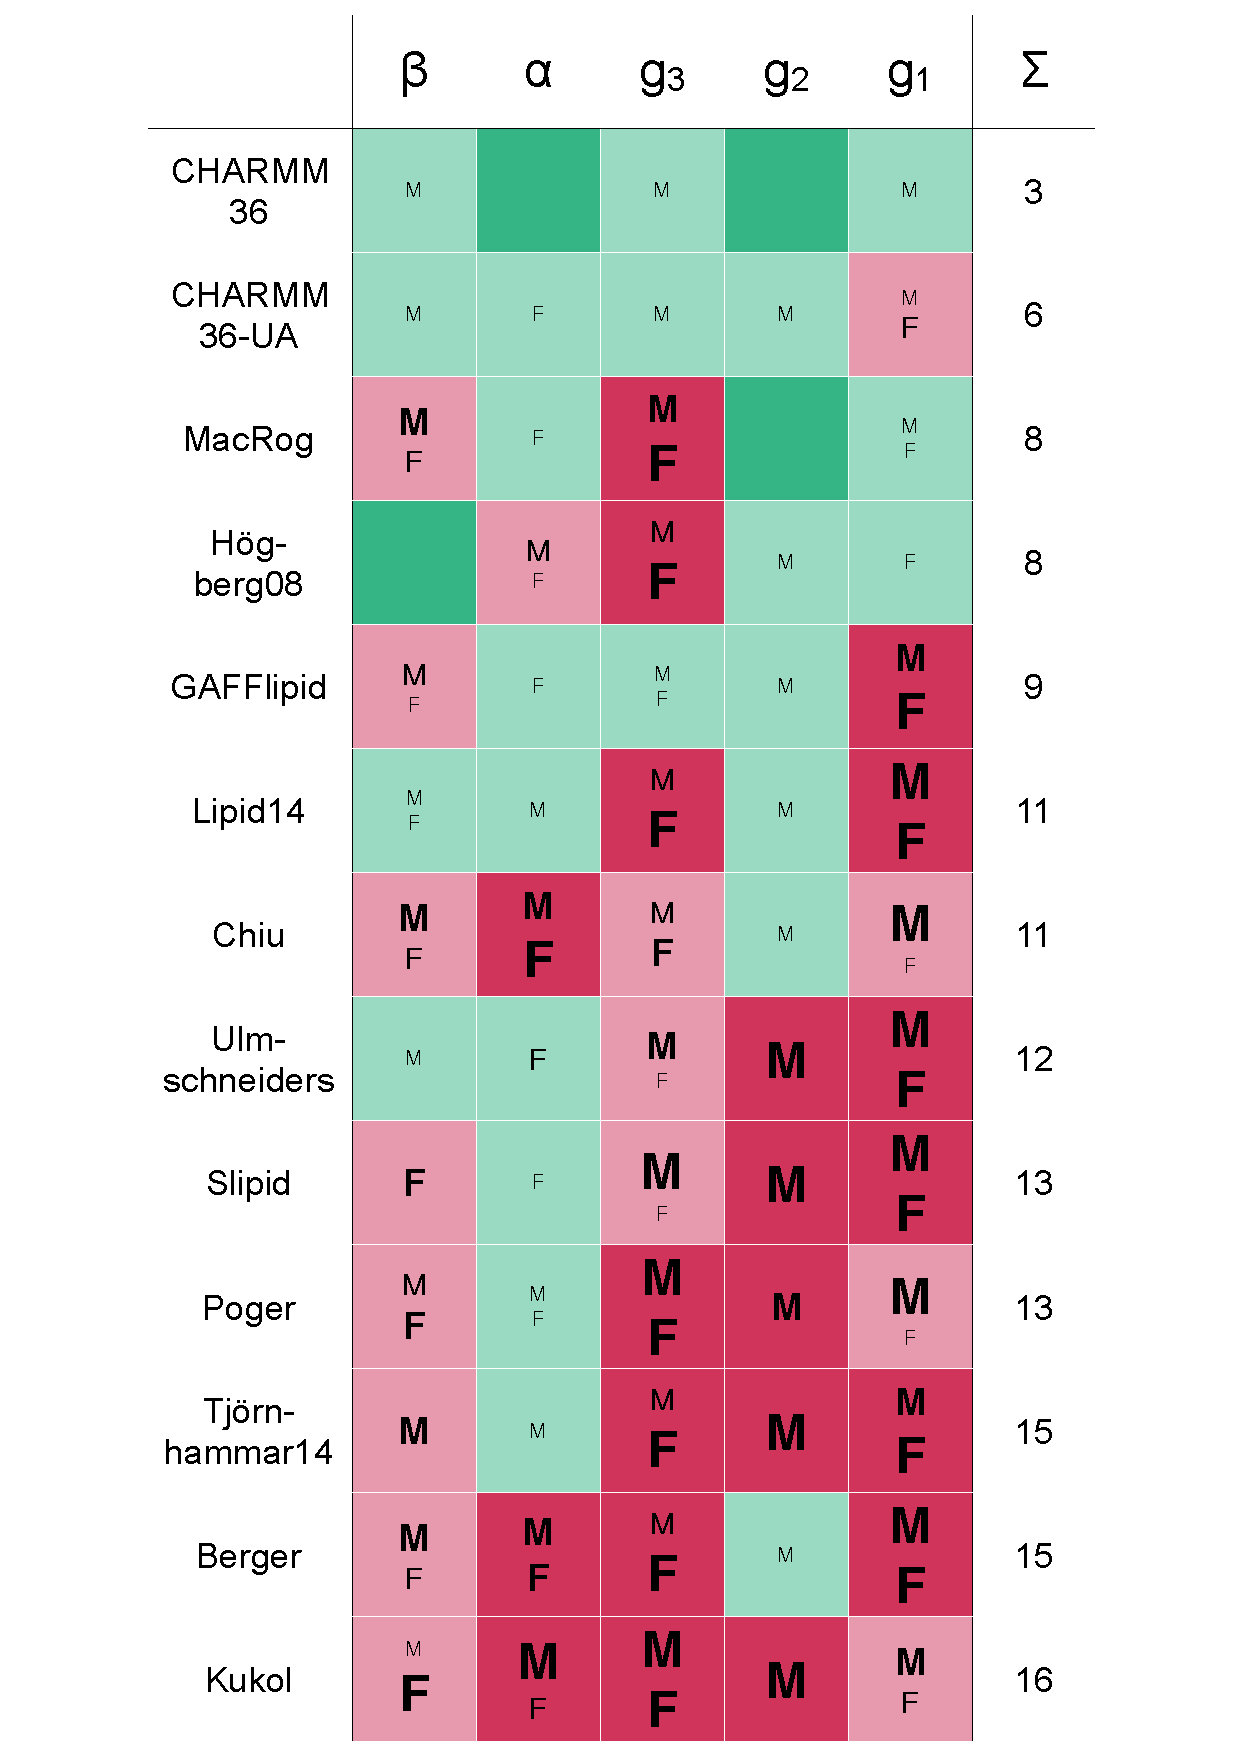
\includegraphics[width=8.6cm]{../DATAreportediINblog/comparisonTable.pdf}
  \newline
  \caption{\label{FullHydrationComparisonTable}
Rough subjective ranking of force fields based on Fig.~\ref{HGorderparameters}.
%
Here "M" indicates a magnitude problem, "F" a forking problem;
letter size increases with problem severity.
%
Color scheme:
"within experimental error" (dark green),
"almost within experimental error" (light green),
"clear deviation from experiments" (light red), and
"major deviation from experiments" (dark red).
%
The $\Sigma$-column shows the total deviation of the force field,
when individual carbons are given weights of 0 (matches experiment), 1, 2, and 4 (major deviation).
%
For full details of the assessment, see Supporting Information.
} 
\end{figure}

None of the studied force fields fulfils these criteria completely, however CHARMM36 is close. 
This is not surprising since the dihedral potentials in this model are tuned to reproduce these 
parameters better against experiments~\cite{klauda10}.
The next models in the list are CHARMM36-UA~\cite{henin08,lee14} and H\"ogberg08~\cite{hogberg08} which is also not surprising since
these models are using CHARMM bonded potentials for glycerol backbone and choline. The fourth and the fifth models in the list, MacRog~\cite{maciejewski14} and
GAFFlipid~\cite{dickson12}, have independently determined dihedral potentials. All the models based on Gromos potentials and Slipids perform less well.
In the present work we subject the CHARMM36, MacRog, GAFFlipid and Berger-POPC-07 to a more careful comparison including the sterospecific labeling  
(Fig.~\ref{HGorderparameters2}), and atomistic level structure and responses to the dehydration and cholesterol content in the following sections.
These models are selected for more detailed studies since they are the best representatives of different dihedral potential parametrization techniques 
(CHARMM36, MacRog, GAFFlipid), and the Berger based models are the most used lipid models in the literature.


\subsection{Full hydration: Atomistic resolution structures in different models}

The results in the previous section revealed significant differences of the glycerol backbone and choline headgroup
order parameters between different molecular dynamics simulation models.
However, it is not straightforward to conclude which kind of structural differences (if any)
between the models the results indicate, because the mapping from the order parameters to the 
structure is not unique. In this section we demonstrate that 1) the differences in order parameters
indicate significantly different structural sampling strongly correlating with the dihedral angles of the related bonds,
and that 2) the comparison between experimental and simulated order parameters can be used to exclude
nonrealistic structural samping in molecular dynamics simulations. The demonstration is done for 
the dihedral angles defined by the g$_3$-g$_2$-g$_1$-O(\textit{sn}-1) segments in the glycerol backbone and 
the N-$\beta$-$\alpha$-O segments in the headgroup. These dihedrals were chosen for demonstration, because 
significant differences between the models are observed around these segments in Fig.~\ref{HGorderparameters2}.
We note that performing a similar comparison through all the dihedrals in all the 13 models would probably give highly useful
information on how to improve the accuracy of the models yet this is beyond the scope of the current report. 

The dihedral angle distributions for the  g$_3$-g$_2$-g$_1$-O(\textit{sn}-1) dihedral calculated from different models are
shown in Fig.~\ref{dihDISTS}. The distribution is qualitatively different for the Berger-POPC-07 model, showing a maximum in 
the gauche$^+$-conformation (60$^o$) compared to all the other models showing a maximum in the anti-conformation (180$^o$).
The distributions in all the other models have the same general features, the main difference being that the
fraction of configurations in the gauche$^-$-conformation (-60$^o$) is zero for the MacRog, detectable for the CHARMM36 and
equally large to the gauche$^+$ fraction in GAFFlipid. From the results we conclude that most likely the wrongly sampled
dihedral angle for the g$_2$-g$_1$ bond explains the significant discrepancy to the experimental order parameters
for the g$_1$ segment in the Berger-POPC-07 model (Fig.~\ref{HGorderparameters2}). 
In conclusion, models preferring the anti conformation for this dihedral give more realistic order parameters and
this is in agreement with previous crystal structure and $^1$H NMR studies~\cite{hauser80,hauser81,hauser81b,hauser88,pascher92,marsh06}.
\begin{figure}[]
  \centering
  \includegraphics[width=8.6cm]{../Fig/g1-g2_Cdihs2.eps}
  \caption{\label{dihDISTS}
    Dihedral angle distributions for g$_3$-g$_2$-g$_1$-O(\textit{sn}-1) dihedral from different models (POPC bilayer in full hydration).
      } 
\end{figure}

The dihedral angle distribution for the  N-$\beta$-$\alpha$-O dihedral calculated from the same four models is 
shown in Fig.~\ref{dihDISTS2}. Also for this dihedral there are significant differences in the gauche--anti fractions.
The gauche conformations are dominant in the CHARMM36, in MacRog there are only anti conformations present,
and in the Berger-POPC-07 and GAFFlipid gauche and anti conformations have equal probabilities. 
On the other hand, comparison of $\alpha$ and $\beta$ order parameters in Fig.~\ref{HGorderparameters2}
reveals that for these carbons the CHARMM36 is closest to the experimental results and it is also the only model that has the correct
sign (negative) for the $\beta$ order parameter. This result is again in agreement with previous 
crystal structure, $^1$H NMR and Raman spectroscopy studies~\cite{hauser80,hauser81,hauser81b,akutsu81b} which suggest that
this dihedral is in the gauche conformation in the absence of ions.

\begin{figure}[]
  \centering
  \includegraphics[width=8.6cm]{../Fig/a-bDIHS2.eps}
  \caption{\label{dihDISTS2}
    Dihedral angle distributions for N-$\beta$-$\alpha$-O dihedral from different models (POPC bilayer in full hydration).
  } 
\end{figure}

The used examples show that the glycerol backbone and headgroup order parameters reflect the atomistic resolution structure
and that the comparison with experiments allows the assessment of the quality of the suggested structure. We were able to pinpoint
specific problems in the structures in different models and suggest potential improvement strategies.
If the improved atomistic
molecular dynamics simulation model reproduced the order parameters and other experimental observables 
(like $^{31}$P chemical shift anisotropy~\cite{chowdhary13} and $^{31}$P-$^{13}$C dipolar couplings~\cite{prakash10})
with experimental accuracy, it would give an interpretation for the atomistic resolution structure of the glycerol backbone and 
choline~\cite{seelig77b,skarjune79,jacobs80,davis83,akutsu91,hong95b,semchyschyn04}. The research along these lines is left, however,
for future studies.


\subsection{Response to dehydration and cholesterol content}
In addition to pure phosphatidylcholine bilayers at full hydration, the choline headgroup order parameters
have been measured under various different conditions~\cite{gally75,brown77,brown78,akutsu81,altenbach84,scherer89,bechinger91,ulrich94,dvinskikh05b,castro08,kapla12,ferreira13}.
Also the order parameters for the glycerol backbone have been measured with $^1$H-$^{13}$C NMR in dehydrated conditions~\cite{dvinskikh05b}, and as a function 
of anesthetics~\cite{castro08} and glycolipids~\cite{kapla12} for DMPC, and as a function of cholesterol 
concentration for POPC~\cite{ferreira13}. Due to the high resolution in the NMR (especially $^2$H NMR) experiments,
even very small order parameter changes resulting from the varying conditions can be measured 
(see Ref.~\citenum{accuracyPOST} for more discussion.) 
However, as already discussed above, it is not simple to deduce 
the structural changes from order parameter changes~\cite{akutsu91,semchyschyn04}. Consequently, comparison of the order parameters
between simulations and experiments in different conditions can be used to assess the quality of the force field 
in different situations, and, if the quality is good, to interpret the structural changes in experiments.
Here we exemplify such comparison for a lipid bilayer under low hydration levels and when varying amounts of cholesterol is included in the bilayer. 
The interaction between ions and a phosphatidylcholine bilayer will be discussed in a separate study~\cite{ionpaper}.

\subsubsection{Phospholipid bilayer with low hydration level}
Fig.~\ref{ordPhydr} shows the published~\cite{dvinskikh05b,ulrich94,bechinger91} experimental order parameters
for the glycerol backbone and choline as a function of hydration level.
Despite slight differences in temperature and acyl chain composition,
the three independently reported data sets for the choline ($\beta$ and $\alpha$) segments agree well with each other:
Both order parameters increase with decreasing hydration level.
The glycerol backbone order parameters (g$_{3}$, g$_{2}$, g$_{1}$), in contrast,
have been observed~\cite{dvinskikh05b} to slightly decrease with dehydration.
Note that the original experiments~\cite{dvinskikh05b,ulrich94,bechinger91} measured only 
absolute values, but here
we included the signs measured in separate studies~\cite{hong95a,hong95b,gross97}. 
Consequently, the negative $\beta$ order parameter actually increases with dehydration 
as its absolute value decreases~\cite{dvinskikh05b,ulrich94,bechinger91}.
\begin{figure}[]
  \centering
  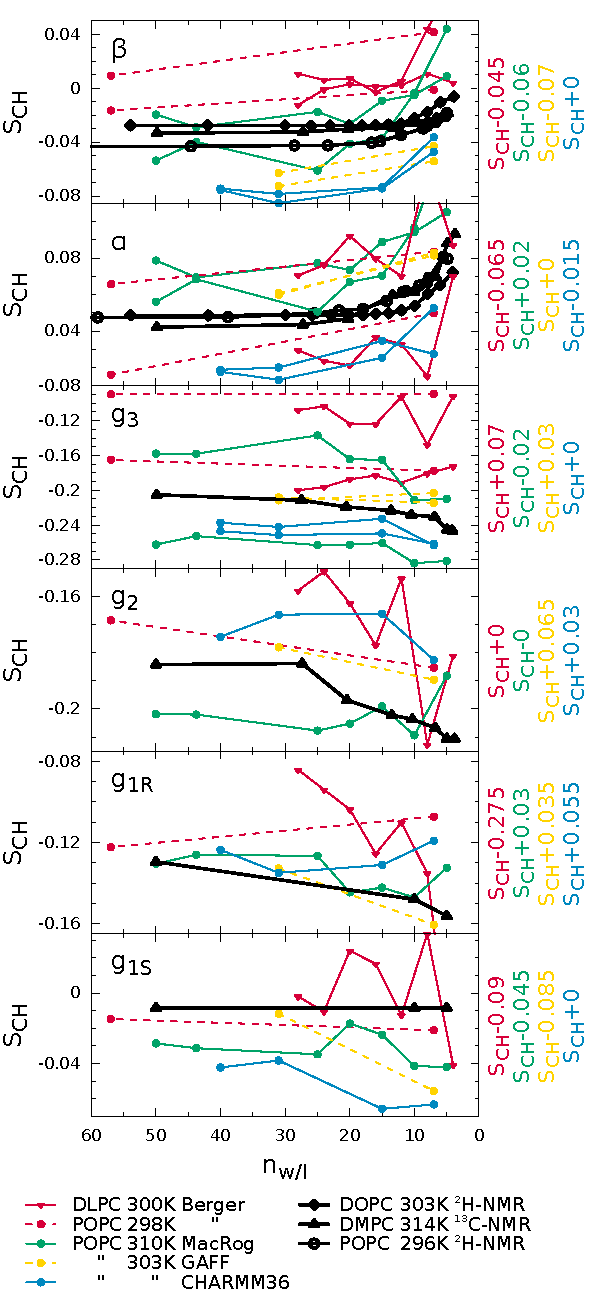
\includegraphics[width=7.3cm]{../DATAreportediINblog/dehydration.pdf}
    \caption{\label{ordPhydr}
    The effect of dehydration on glycerol and choline order parameters in experiments.
    The magnitudes of order parameters are measured for DMPC ($^1$H-$^{13}$C NMR) at 314~K~\cite{dvinskikh05b}, 
    for POPC ($^2$H NMR) at 296~K~\cite{bechinger91} and for DOPC ($^2$H NMR) at 303~K~\cite{ulrich94}. 
    The signs are based on the measurements by Hong et al.~\cite{hong95a,hong95b} 
    and Gross et al.~\cite{gross97}.
    Note that to elucidate the relative change as a function of hydration level, the simulation results were vertically shifted; 
    the shift magnitudes for each of the force fields are listed (SCH+shift) in the y-label.
  }
\end{figure}

Lipid bilayer dehydration has been studied also with molecular dynamics simulations~\cite{mashl01,pertsin05,pertsin07,eun09,eun10,schneck12},
typically motivated by the  discussion concerning the origin of the ``hydration repulsion''~\cite{israelachvili,israelachvili96,sparr11}.
Only one~\cite{mashl01} of these studies, however, compared their simulation model to the experimental choline and glycerol backbone
order parameters.
Fig.~\ref{ordPhydr} shows these order parameters as a function of hydration level for the CHARMM36, 
MacRog and GAFFlipid models (having the most realistic atomistic resolution structures) and a Berger-based model 
(which is the most used lipid model);
note that the simulation results have been vertically shifted to ease the comparison with experimental response to dehydration.
Despite of some fluctuations, the increase of the choline ($\beta$ and $\alpha$) order parameters is seen in all four
models. The response of the choline order parameters to dehydration can, therefore, be
interpreted to qualitatively agree with experiments.
The situation is significantly more complicated for the glycerol backbone: 
None of the four models produced the experimentally seen trends
in all the (g$_{3}$, g$_{2}$, g$_{1}$) segments.

The qualitative agreement of the $\alpha$ and $\beta$ order parameters with experiments in all four simulation models (Fig.~\ref{ordPhydr}) indicates that,
despite the unrealistic structures at full hydration (Figs.~\ref{HGorderparameters} and~\ref{FullHydrationComparisonTable}),
the structural response of the choline headgroup to dehydration is somewhat realistic.
A likely explanation is that as the interlamellar space shrinks with dehydration, the whole choline group
orients more parallel to the membrane.
Indeed, upon dehydration the angle between P--N (phoshate phosphorus to choline nitrogen) vector and membrane normal increases for
all the four models (Fig.~\ref{PNangle}). However,
the amount of increase depends on the model. Especially the DLPC simulations with Berger model
predict significantly stronger P--N vector tilt than the other models. The Berger model
has also generally larger P--N vector angles and its choline order parameters are more off from
experiments than the other three models (Fig.~\ref{HGorderparameters2}). Thus the relatively modest tilting with dehydration
predicted by MacRog, CHARMM36 and GAFFlipid is probably more realistic.

It must be stressed that in the models
incapable of reproducing the experimental order parameters the free energy landscape is not correct. Thus
even though the order parameter response to dehydration is qualitatively correct,
the energetic response is likely to be incorrect.
This may have some influence on dehydration energetic calculations made using the Berger model~\cite{eun09,schneck12}.
\begin{figure}[]
  \centering
  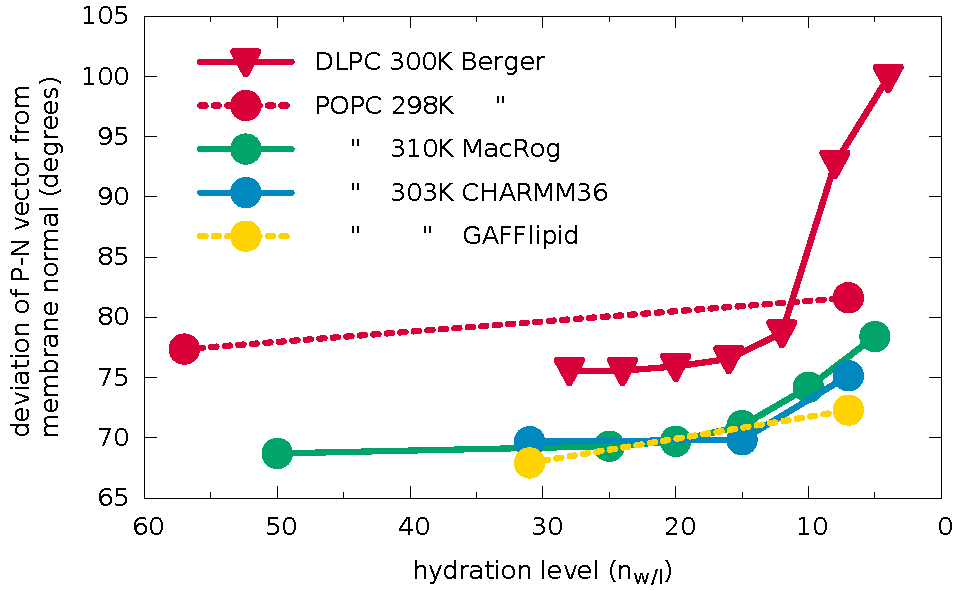
\includegraphics[width=8.6cm]{../Fig/dehydrationPN.pdf}

  \caption{\label{PNangle}
    The average angle between membrane normal and P--N vector as function of
    hydration level calculated from different simulations.
  }
\end{figure}

The response of the glycerol backbone seems to be more subtle than that of the choline headgroup;
none of the four models reproduced the experimental trends upon dehydration with enough accuracy to invite a
structural interpretation.

\subsubsection{Cholesterol-containing phospholipid bilayer}
As cholesterol is abundant in biological membranes and
has been suggested to be an important player, for example, in domain formation~\cite{simons04,somerharju09},
phospholipid--cholesterol interactions have been extensively studied with theoretical~\cite{huang99,zhu07,rog09,alwarawrah12} and
experimental~\cite{brown78,marsh10,ferreira13,marsh13} methods.
It is widely agreed that cholesterol orders lipid acyl tails and thus decreases the area per molecule (condensing effect),
but its influence on the lipid headgroup and glycerol backbone remains debated~\cite{huang99,simons04,somerharju09}.
It has been suggested, for example, that the surrounding phospholipids shield cholesterol from exposure to water by 
reorienting their headgroups (``umbrella model'')~\cite{huang99} or that cholesterol acts as a spacer between the headgroups to increase 
their entropy and dynamics (``superlattice model'')~\cite{somerharju09}. 
Molecular dynamics simulations have supported both
the umbrella~\cite{alwarawrah12} as well as the superlattice~\cite{zhu07} model,
in addition to suggesting specific interactions of cholesterol with the glycerol backbone~\cite{rog09}.
In these studies~\cite{zhu07,rog09,alwarawrah12}
the responses of the glycerol backbone and choline headgroup 
to increasing cholesterol content were not, however, compared to experiments. 

Fig.~\ref{ordPchol} shows the responses of the choline headgroup ($\beta$ and $\alpha$)
order parameters of POPC (measured by $^1$H-$^{13}$C NMR~\cite{ferreira13}) and DPPC
($^{2}$H NMR~\cite{brown78}) to increasing cholesterol content.
Again, the two independent data sets agree very well:
Only very modest ($\Delta S_\mathrm{CH}<0.03$) changes occur in  the choline order parameters as cholesterol content
increases from 0 to 60\%.
The extreme sensitivity of the
high resolution $^{2}$H NMR experiments
is beautifully demonstrated by the measurable~\cite{brown78}
(but barely visible on the scale used in Fig.~\ref{ordPchol})
cholesterol-induced forking of the $\alpha$ order parameter.

We note that the modest ($\Delta S_\mathrm{CH}<0.02$ for g$_1$; $<0.04$ for g$_2$, g$_3$; see Fig.~\ref{ordPchol})
effects of cholesterol
on the glycerol backbone order parameters of POPC
measured by $^1$H-$^{13}$C NMR~\cite{ferreira13}
agree well with the results for phosphatidylethanolamine (PE) measured by $^{2}$H NMR~\cite{ghosh82}.
This further supports the ideas that the glycerol backbone structural behaviour is independent of the
headgroup composition~\cite{gally81} and that the headgroup structure is largely independent of the acyl chain region content unless
charges are present~\cite{scherer87}.
\begin{figure}[]
  \centering
  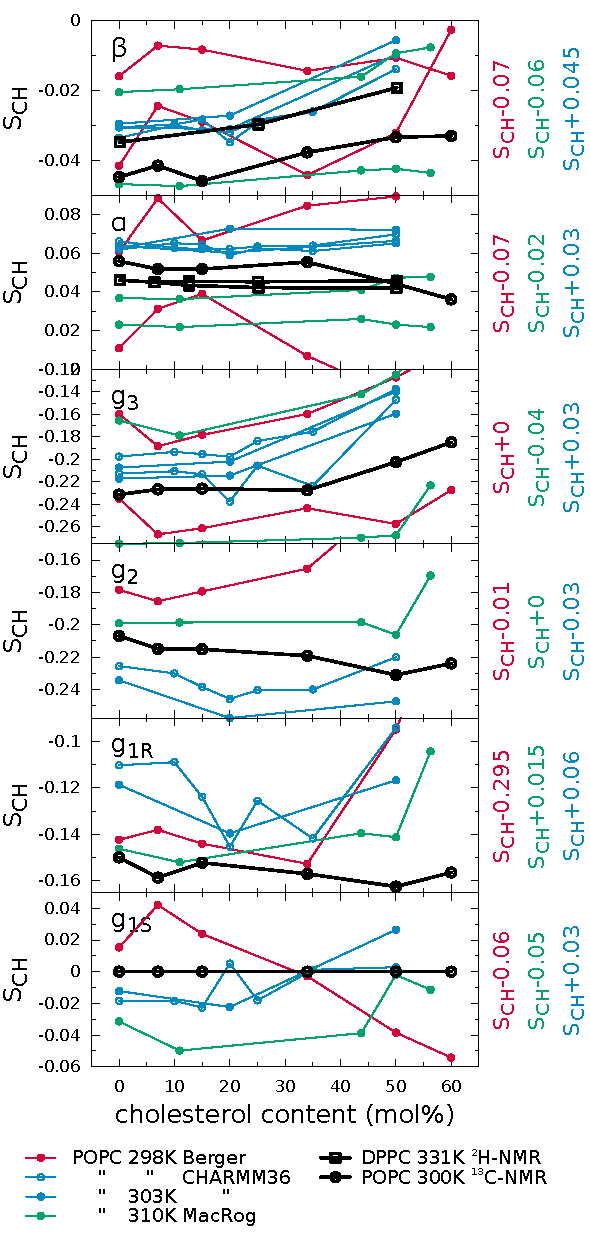
\includegraphics[width=7.3cm]{../DATAreportediINblog/cholesterolization_lp.pdf}
%    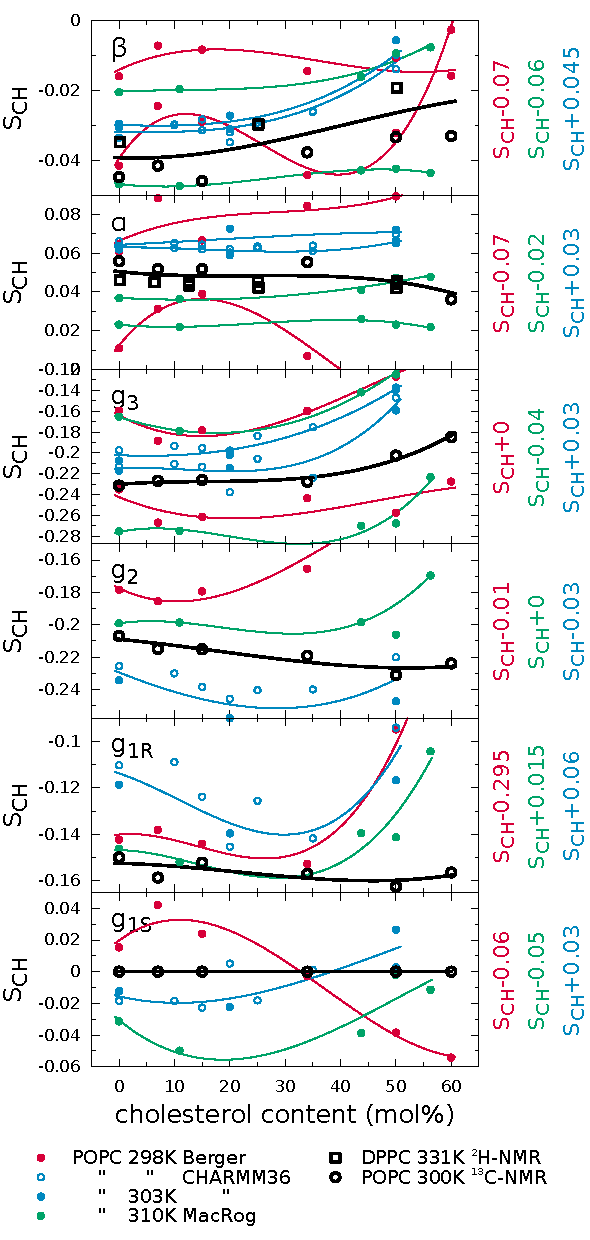
\includegraphics[width=7.3cm]{../DATAreportediINblog/cholesterolization_smooth.pdf}
  \caption{\label{ordPchol}
    The effect of cholesterol content on the glycerol backbone and choline order parameters in experiments~\cite{brown78,ferreira13} and simulations
    with the Berger-POPC-07/H\"oltje-CHOL-13, CHARMM36 and MacRog force fields. The signs in the experimental values are based on the measurements by Hong et al.~\cite{hong95a,hong95b} 
    and Gross et al.~\cite{gross97}.  Most order parameters from Berger-POPC-07/H\"oltje-CHOL-13 model for g$_1$ are beoynd the y-axis scale.
    In order to elucidate the relative change as a function of cholesterol content, the simulation results were vertically shifted; 
    the shift magnitudes for each of the force fields are listed (SCH+shift) in the y-label.
}
\end{figure}

In addition to the experimental data, Fig.~\ref{ordPchol} shows
our results for the CHARMM36 and MacRog force fields
and the previously published~\cite{ferreira13}
Berger-POPC-07/H\"oltje-CHOL-13 results.
Note that the simulation data are shifted vertically to ease comparison with experimental responses.
As previously pointed out~\cite{ferreira13}, the Berger-based model
seriously exaggerates the effect of cholesterol on the phospholipid glycerol backbone and choline headgroup.
In comparison, the choline and glycerol backbone responses of CHARMM36 and MacRog are in better qualitative 
agreement with experiments. 
Therefore, to resolve the nature of cholesterol-induced structural changes,
we calculated from CHARMM36 the glycerol backbone orientation and dihedral angle distributions
at various cholesterol contents (Supporting Information). The only detectable changes
are the small decrease of gauche(-) and increase of gaughe(+) probability of 
the g$_3$-g$_2$-g$_1$-O(\textit{sn}-1) dihedral and slight (less than 5 degrees) change
in the glycerol backbone orientation. In conclusion, our results suggest that the significant 
effects of cholesterol on lipid conformations observed in simulations~\cite{zhu07,rog09,alwarawrah12} 
are overestimated by the computational models used;
cholesterol only induces very small structural changes in the glycerol backbone.

Finally, it is important to note that the CHARMM36 force field parameters (glycerol backbone dihedral potentials)
have been tuned to reproduce the experimental order parameters at full hydration~\cite{klauda10}. 
This approach introduces a risk of overfitting, which would manifest itself as wrong responses to changing conditions. 
Interestingly, according to our results, tuning did not lead to overfitting problems as far as dehydration or cholesterol content are considered. 


\pagebreak
\section{Conclusions}
The atomistic resolution structures sampled by the glycerol backbone and choline headgroup
in phoshatidylcholine bilayers are not known despite of vast amount of accurate experimental
data. An atomistic resolution molecular dynamics simulation model that would reproduce the
experimental data would automatically resolve the structures, thus giving an unprecedently detailed interpretation of the experimental data.
In this work we have collected and reviewed the experimental C--H bond vector order
parameters available in the literature. These accurate experimental data are then compared to 13
different atomistic resolution simulation models for a fully hydrated lipid bilayer system, followed by bilayers dehydrated to different extents, and
finally bilayers containing various amounts of cholesterol. We are led to the following four main conclusions:

(1) The C--H bond order parameters measured with different NMR techniques are consistent.
By combining the experimental results from various sources we concluded
that the order parameters for each C--H bond are known with a quantitative accuracy of $\pm$0.02.

(2) Comparison of order parameters between experiments and different atomistic resolution models 
together with structural analysis showed that the order parameters can be used
to judge the structural accuracy of a model. Thus the combination of atomistic resolution 
molecular dynamics simulations and NMR experiments can be used to resolve the atomistic resolution
structures of biomolecules in biologically relevant conditions. 
This approach can be extended from lipids to, for example, membrane proteins.

(3) The review of previous experimental results revealed that when a bilayer is dehydrated the 
choline order parameters increase. Our simulations suggested that
this can be explained by the P--N vector tilting more parallel to the membrane. 
This strongly supports and complements the idea that charge-induced choline tilting
can be measured using order parameter changes~\cite{ionpaper,scherer89}.

(4) Only modest changes of glycerol backbone and choline order parameters are observed experimentally with increasing cholesterol content.
When interpreted using the computational lipid model that we found to have the most realistic response to cholesterol,
this observation means that cholesterol induces only minor changes in (the g$_3$-g$_2$-g$_1$-O(sn-1)
dihedral of the glycerol backbone, in other words, there is no major conformational change of the lipid.

(+) Besides these four main conclusions, we note that we have created the most extensive
publicly available collection of molecular dynamics simulation trajectories of lipid bilayers
(\url{https://zenodo.org/collection/user-nmrlipids}). The mere existence of
this collection opens up numerous possibilities for unforeseen analyses, such as data mining,
and rapid testing of ideas with
much less computational effort than previously required.

In general, we conclude that in order to fully utilize the potential of atomistic-resolution classical molecular dynamics simulations
in the structural interpretation of high resolution NMR data~\cite{ferreira14} for lipid bilayers, one must  
improve the phoshatidylcholine glycerol backbone and choline headgroup parameters of the existing force fields.

This work has been done as a fully open collaboration, using \url{nmrlipids.blogspot.fi} as the communication
platform. All the scientific contributions have been communicated publicly through this blog~\cite{nmrlipids}.

%%%%%%%%%%%%%%%%%%%%%%%%%%%%%%%%%%%%%%%%%%%%%%%%%%%%%%%%%%%%%%%%%%%%%
%% The "Acknowledgement" section can be given in all manuscript
%% classes.  This should be given within the "acknowledgement"
%% environment, which will make the correct section or running title.
%%%%%%%%%%%%%%%%%%%%%%%%%%%%%%%%%%%%%%%%%%%%%%%%%%%%%%%%%%%%%%%%%%%%%
\begin{acknowledgement}

We acknowledge all the discussion participants at nmrlipids.blogspot.fi.
AB and CL acknowledges financial support from the French National Research Agency
(ANR: “Biolubrication by phospholipid membranes” Bioub2012) and
computing time allocation from P{\^o}le Scientifique de Mod{\'e}lisation Num{\'e}rique from the ENS Lyon (PSMN),
and Centre Informatique National de l'Enseignement Sup{\'e}rieur (CINES, Montpelier, France)
(Project c2015096850).
FFR acknowledges CONACYT and DGAPA UNAM IG100513
for financial support, Cluster H\'ibrido de Superc\'omputo Xiuhcoatl - CINVESTAV and Miztli - UNAM for computational resources. 
MJ and JT acknowledge and CSC - IT Center for Science for computational resources (project number tty3979).
MJ also acknowledges the Finnish Doctoral Programme in Computational Sciences (FICS) for funding.
JT, MJ, TR and WK acknowledge the funding from the Academy of Finland (Centre of Excellence program) 
and the European Research Council (Advanced Grant project CROWDED-PRO-LIPIDS).
WK acknowledges CSC -- IT Centre for Science (Espoo, Finland) for excellent computational resources (project number tty3995).
MSM acknowledges financial support from the Volkswagen Foundation (86110).
LM acknowledges funding proved by the Institut national de la sant\'e et de la recherche m\'edicale (INSERM).
JM acknowledges CSC -- IT Center for Science for computational resources.
OHSO acknowledges Tiago Ferreira and Paavo Kinnunen for useful discussions, 
the Emil Aaltonen foundation for financial support, 
Aalto Science -- IT project and CSC -- IT Center for Science for computational resources. 
HS acknowleges Catherine Etchebest and St\'ephane T\'eletch\'ea for useful discussions and continued support, the HPC 
resources granted from GENCI-CINES (Grant 2014-c2014077209) and computer facilities provided by R\'egion Ile de France and INTS (SESAME 2009 project).

\end{acknowledgement}

%%%%%%%%%%%%%%%%%%%%%%%%%%%%%%%%%%%%%%%%%%%%%%%%%%%%%%%%%%%%%%%%%%%%%
%% The same is true for Supporting Information, which should use the
%% suppinfo environment.
%%%%%%%%%%%%%%%%%%%%%%%%%%%%%%%%%%%%%%%%%%%%%%%%%%%%%%%%%%%%%%%%%%%%%
\begin{suppinfo}

Simulation and analysis details, two figures, and author contributions.

%This will usually read something like: ``Experimental procedures and
%characterization data for all new compounds. The class will
%automatically add a sentence pointing to the information on-line:

\end{suppinfo}

%%%%%%%%%%%%%%%%%%%%%%%%%%%%%%%%%%%%%%%%%%%%%%%%%%%%%%%%%%%%%%%%%%%%%
%% The appropriate \bibliography command should be placed here.
%% Notice that the class file automatically sets \bibliographystyle
%% and also names the section correctly.
%%%%%%%%%%%%%%%%%%%%%%%%%%%%%%%%%%%%%%%%%%%%%%%%%%%%%%%%%%%%%%%%%%%%%


\bibliography{refs}

\end{document}
